% -*- root: ../Economia.tex -*-
\section{Modelos de un período}
\begin{problem}[1]
El subyacente $S$ vale hoy 60 \texteuro y el modelo que hemos definido prevé, para el tiempo siguiente, un nivel alto en 65 \texteuro y un nivel bajo en 55 \texteuro. El tipo libre de riesgo para el período es del 3\%.
\ppart Calcular la probabilidad riesgo neutro del estado alto de la economía.
\ppart Calcular el valor de una put con precio de ejercicio en 60 \texteuro.
\ppart Misma pregunta si el tipo libre de riesgo, para la composición continua, es ahora del 6\% y el tiempo hasta vencimiento es de seis meses.

\solution

\spart

La situación que descibe el problema puede representarse mediante el siguiente diagrama:

\begin{minipage}{0.48\textwidth}
\begin{center}
\begin{tikzpicture}[->,>=stealth',shorten >=1pt,auto,node distance=2.8cm,
                    semithick]
  %\tikzstyle{every state}=[fill=red,draw=none,text=white]

  \node[state] (A)                    {$S_0$};
  \node[state] (B) [above right of=A] {$aS_0$};
  \node[state] (C) [below right of=A] {$bS_0$};


  \path (A) edge node {q} (B)
  		    edge node {1-q} (C);
\end{tikzpicture}
\end{center}
\end{minipage}
\begin{minipage}{0.48\textwidth}
Siendo en este caso concreto
\[\begin{array}{l}
S_0 = 60 \\
aS_0 = 65 \implies a = 1.08 \\
bS_0 = 55 \implies b = 0.92
\end{array}\]
\end{minipage}

Lo primero que debemos hacer es calcular la probabilidad riesgo neutro, que es aquella que hace que se cumpla la conidición de martingala.

La condición de martingala se escribe como:
\[V_0(\varphi) = \tilde{V}_0(\varphi) = \esp[Q]{\tilde{V}_1(\varphi)}\]

Vamos a forzar que se cumpla esta conidción para despejar el valor de $q$ que buscamos. Para ello suponemos la estrategia trivial $\varphi=(\varphi_1) =(1)$.

\[\esp[Q]{\tilde{V}_1(\varphi)} = \frac{q\cdot aS_0 + (1-q)\cdot bS_0}{S_1^0} = \frac{65q + (1-q)55}{1+r} = \frac{10q+55}{1.03}\]

Por otro lado sabemos que $V_0(\varphi) = 60$ con lo que igualando llegamos a:
\[\frac{10q+55}{1.03} = 60 \implies 10q = 6.8 \implies q = 0.68 \]

\spart

Una \concept{put} es un contrato que da el derecho a vender en tiempo 1 una acción de $S$ por $K$ euros.

Suponiendo que no hubiera ningún tipo de tasa ni impuesto extra que pagar (suposición que no es cierta en los mercados reales) el precio o coste de una put puede calcularse como su valor en el instante $t=0$.

Teniendo los mismos estados del apartado anterior con sus mismos valores y siendo el precio de ejercicio $K=60$ \texteuro (el precio al que garantizamos vender en el futuro) podemos ver que en el estado alto tenemos un valor $X(ω_1)=0$ y en el caso bajo $X(ω_2)=K-bS_0$.

Conociendo las probabilidades riesgo neutras, que calculamos en el aprtado anterior, podemos calcular el valor inicial de la put con la misma fórmula usada en el apartado anterior:
\[P_0 = V_0(\varphi) = \tilde{V}_0(\varphi) = \esp[Q]{\tilde{V}_1(\varphi)} = (1-q) \frac{K-bS_0}{1+r} = 0.32 \cdot \frac{60-55}{1.03}=1.55\]

\spart

Hasta ahora lo que hemos visto es que tenemos un tipo de interes simple que consiste en que nos perstan una cantidad $X$ con un interés $r$ y al final del ejercicio devolvemos la cantidad prestada más los intereses, es decir, ent $t=1$ pagamos
\[(1+r)X\]

No obstante, podríamos considerar que en el instante $t=1/2$ pagamos los intereses correspondientes a 6 meses y en $t=1$ pagamos los intereses de los segundos 6 meses y, además, devolvemos todo el préstamos inicial. En esta ocasión estaríamos pagando
\[\left(1+\frac{r}{2}\right)^2\]

En general, si dividimos los pagos en $n$ plazos estamos pagando
\[\left( 1 + \frac{r}{n} \right)^n\]

Es sencillo ver que si extendemos esta distribución de prestamos hasta considerar intervalos infinitamente pequeños llegamos a una \concept{comosición continua} donde la función que mide lo que debemos pagar se corresponde con una exponencial. Es decir, tendiendo $n$ al infinito lo que estamos pagando es:
\[e^{rt}\cdot X\]

Por tanto, lo único que debemos hacer para trabajar en este tipo de casos es sutituir las operaciones que realizábamos con respecto a $1+r$ al trabajar con precios descontados, por las mismas operaciones respecto a $e^{rt}$.

Puesto que estamos considerando vencimiento de 6 meses tendremos:
\[P_0 = V_0(\varphi) = \tilde{V}_0(\varphi) = \esp[Q]{\tilde{V}_1(\varphi)} = (1-q) \frac{K-bS_0}{e^{rt}} = 0.32 \cdot \frac{60-55}{e^{0.06\cdot 0.5}}=1.55\]
\end{problem}

\begin{problem}[2]
El subyacente $S$ vale hoy 10 \texteuro y el model definido prevé, para el tiempo siguiente, un nivel alto en 12 \texteuro y un nivel bajo en 9 \texteuro. El tipo libre de riesgo para el período es del 10\%. Consideramos un derivado $X$ que pagará el cuadrado del valor $S_1$ a vencimineto.

\ppart ¿Cuál es la cartera de cobertura para dicho derivado?
\ppart Calcular el valor de dicho derivado en 0.
\ppart Calcular el valor de una call sobre este derivado con un precio de ejercicio de 100.
\ppart Un segundo análisis le lleva a pensar que los dos estados futuros del modelo han de ser 10.5 y 9.5 (permaneciendo inalterado el tipo libre de riesgo). ¿Es el nuevo modelo viable (libre de arbitrajes)? [Intenta calcular la probabilidad riesgo neutro del estado alto]

\solution

\spart

La \concept{cartera de cobertura} no es más que aquella que a vencimiento nos garantiza los mismos resultados que el derivado que queremos cubrir.

Tenemos por ahora un derivado $S^0$ que es la \concept{cuenta bancaria} que tiene un interés fijo y conocido; y el activo descrito por el enunciado, $S$, que llamaremos $S^1$ que sigue el siguiente esquema

\begin{minipage}{0.48\textwidth}
\begin{center}
\begin{tikzpicture}[->,>=stealth',shorten >=1pt,auto,node distance=2.8cm,
                    semithick]
  %\tikzstyle{every state}=[fill=red,draw=none,text=white]

  \node[state] (A)                    {$S_0^1$};
  \node[state] (B) [above right of=A] {$aS_0^1$};
  \node[state] (C) [below right of=A] {$bS_0^1$};


  \path (A) edge node {q} (B)
  		    edge node {1-q} (C);
\end{tikzpicture}
\end{center}
\end{minipage}
\begin{minipage}{0.48\textwidth}
Siendo en este caso concreto
\[\begin{array}{l}
S_0^1 = 10 \\
aS_0^1 = 12 \implies a = 1.2 \\
bS_0^1 = 9 \implies b = 0.9
\end{array}\]
\end{minipage}

La estrategia de cobertura será aquella $\varphi=(\varphi_0,\varphi_1)$ compuesta por los activos $S^0$ y $S^1$ que, a vencimiento, nos da los mismos resultados que el activo $X$. Para encontrar esta cartera simplemente debemos resolver la ecuación:
\[\left\{ \begin{array}{l}
\varphi_0(1.1) + \varphi_1\cdot 12 = 144 \\
\varphi_0(1.1) + \varphi_1\cdot 9 = 81
\end{array}\right. \implies \varphi_1 = 21 \text{ y } \varphi_0 = -98.18\]

\spart

Para conocer el valor de este derivado en $t=0$ necesitamos conocer cuál es la probabilidad de que se de cada suceso de los planteados para $t=1$.

Vamos a centrarnos en el activo $S^1$ que conocemos. Puesto que \textbf{suponemos que estamos trabajando en una economía libre de arbitrajes} sabemos que existe la \concept{probabilidad riesgo neutro}, que es aquella que garantiza que el valor de precios descontados de una cartera coincida con su valor inicial. Es decir:
\[V_0(\varphi) = \tilde{V}_0(\varphi) = \esp[Q]{\tilde{V}_1(\varphi)}\]

Por tanto, para conocer esta probabilidad sólamente tenemos que resolver la ecuación:
\[10 =  \frac{q\cdot aS_0 + (1-q)\cdot bS_0}{S_1^0} =  \frac{q\cdot 12 + (1-q)\cdot 9}{1.1} = \frac{3q + 9}{1.1} \implies q=0.67\]

Una vez conocemos esta probabilidad, podemos calcular el valor del derivado como valor descontado esperado del mismo:
\[V_0(X) = \frac{qX(ω_1) + (1-q)X(ω_2)}{1+r} = \frac{0.67\cdot 144 + 0.33\cdot 81}{1.1} = 112\]

\spart

Una \concept{call} es un contrato que da derecho a comprar un producto $S$ por $K$ euros en tiempo $t=1$.

En esta ocasión tenemos un precio $K=100$ \texteuro. Para calcular su precio lo único que debemos hacer es considerarlo como un derivado más y aplicar el mismo razonamiento que empleamos al final del apartado anterior.

Con probabilidad $q$ estaremos en el estado alto, por lo que compraremos el derivado de precio 144 \texteuro por los 100 \texteuro acordados en la call. Por otro lado, si estamos en el estado bajo de la economía, optamos por no comprar con lo que no perdemos nada. Por tanto tenemos $X(ω_1)=aS^1_0-K$ y $X(ω_2)=0$. Así tenemos:

\[C_0 = \frac{qX(ω_1) + (1-q)X(ω_2)}{1+r} = \frac{0.67(144-100)}{1.1} = 26.8\]

\spart

Con la nueva situación descrita, y siguiendo la indicación del enunciado, tratamos de calcular la probabilidad riesgo neutro correspondiente. Así tenemos:
\[10 = \frac{10.5q + (1-q)9.5}{1+r} = \frac{q+9.5}{1.1}\implies q=1.5 \]

Evidentemente esta situación no es posible puesto que $q$ es una probabilidad, que no puede ser mayor que 1. Veamos cómo estudiar esta situación.

Si nos fijamos podemos observar que en el estado alto de este activo tenemos un valor menor que el correspondiente a la cuenta bancaria. Aquí surge el arbitraje: nos ponemos en corto con el activo $S$, es decir, vendemos $n$ acciones de $S$ que aún no hemos comprado. El dinero ganado con esta puesta en corto, $10\cdot n$ \texteuro, lo metemos en una cuenta bancaria con tipo libre de riesgo $1.1$.

En $t=1$ debemos comprar las acciones de $S$ al precio que estén para entregarlas que seguro será menor que la cantidad que tenemos en el banco. Por tanto, estamos ganando dinero sin riesgo alguno.
\end{problem}

\begin{problem}[3]
El subyacente $S$ vale hoy 10 \texteuro y el modelo que hemos definido prevé, para el tiempo siguiente, un nivel alto en 12 \texteuro y un nivel bajo en 8 \texteuro. El tipo libre de riesgo para el período es del 5\%. Calcular el valor de una call de precio de ejercicio 11 \texteuro:
\ppart Por no arbitraje

\ppart Por valoración riesgo neutro.
\solution

Empezamos calculando la probabilidad riesgo neutro asociada al estado alto de este modelo. Nuevamente, reutilizamos las fórmulas y los conceptos de los dos ejercicios anteriores. Así tenemos
\[10 = \frac{12q + (1-q)8}{1.05} = \frac{4q+8}{1.05} \implies q=0.63\]

\spart

Vamos a buscar la estrategia de cobertura de este activo que es la call. Así tenemos que resolver el siguiente sistema:

\[\left\{ \begin{array}{l}
\varphi_0(1.05) + \varphi_1\cdot 12 = 1 \\
\varphi_0(1.05) + \varphi_1\cdot 8 = 0
\end{array}\right. \implies \varphi_1 = 0.25 \text{ y } \varphi_0 = -1.9\]

Puesto que estamos bajo la suposición de que nos movemos en una economía libre de arbitrajes, el precio inicial de esta estrategia debe coincidir con el previo actual del activo $X$ (la call).

Así tenemos:
\[C_0 = V_0(\varphi) = \frac{\varphi_0(1+r) + q(\varphi_1 \cdot 12) + (1-q)(\varphi_1\cdot 8)}{1+r} = -1.9 + \frac{0.63 \cdot 0.25\cdot 12 + 0.37 \cdot 0.25 \cdot 8}{1.05}\]
\[C_0 = 0.6\]
\spart

Una vez conocemos la probabilidad riesgo neutro podemos calcular el precio de la call como sigue:
\[C_0 = q\cdot \frac{aS_0 - K}{1+r} = 0.63 \frac{12-11}{1.05} = 0.6\]

Como era de esperar los dos procedimientos nos llevan a la obtención del mismo precio.
\end{problem}

\begin{problem}[4]
La ausencia de oportunidades de arbitraje es una de las exigencias más fuertes que se le pueden hacer al modelo. Una exigencia primera es la ley de un único precio: el modelo no puede asignar dos precios distintos a un mismo subyacente o derivado por una cuestión elemental de consistencia.

\ppart Comprobar que un modelo con $S_0 = 10$ y $S_1(ω_1)=S_1(ω_2)=12$ no satisface la ley de único precio, siendo $r=0.1$.
% Comenté este ejercicio con el profesor y concluimos que era necesario un valor de r que no proporciona el enunciado. Nos inventamos un valor que tuviera sentido.

\ppart ¿Puede dar otro ejemplo?
\solution

\spart
Considerando el activo $S$ descrito en el enunciado, vamos a comprobar cuál es el precio actual de ese activo, atendiendo a sus precios de futuro tanto en el estado alto como en el bajo.

\[S_0 = \frac{qS_1(ω_1) + (1-q)S_1(ω_2)}{1+r} = \frac{12}{1.1}=10.9\]

Es evidente comprobar que este precio inicial no se corresponde con $S_0=10$ por lo que la ley de único precio no se satisface.

\spart

Apoyándonos en el ejercicio anterior, es sencillo ver que el siguiente modelo no cumple la ley de precio único.
\[\left\{\begin{array}{l}
C_0 = 1 \\
K = 11 \\
r = 0.05\\
S_0 = 10 \\
S_1(ω_1) = 12\\
S_2(ω_2) = 8
\end{array}\right.\]


\end{problem}

\begin{problem}[5]
Se dice que una estrategia $\tilde{\varphi}$ domina a otra estrategia $\varphi$ $(\varphi \prec \tilde{\varphi})$ si $V_0=\tilde{V}_0$ y $V_1(w) < \tilde{V}_1(ω)$ para todo $ω \in Ω$.

\ppart Comprobar que en un modelo con $S_0=10$ y $S_1(ω_1)=12$ y $S_1(ω_2) = 8$ con $r=1$ $\varphi=(10,-1)$ es una estrategia dominante,

\ppart Demostrar, sin embargo, que se cumple la ley de un precio.

\ppart Construir un arbitraje
\solution

\spart
\doneby{Pedro}

La estrategia $\varphi = (10,-1)$ tiene un valor inicial:
\[V_0(\varphi)=10-1\cdot 10 = 0\]

Para garantizar que la estrategia es dominante debemos comprobar que cualquier otra estrategia con valor inicial 0 tiene valores finales (tanto en el estado alto como en el bajo) menores que $V_1(\varphi(ω))$.

Dados los activos con los que estamos trabajando (la cuenta sin riesgo y $S$), toda estrategia que tenga valor 0 en $t=0$ será de la forma:
\[\varphi_a = (10a, -a) \text{ con } a \in \ent\]

Para la estrategia dada por el enunciado tenemos:
\[\left\{ \begin{array}{l}
V_1(\varphi(ω_1))= 10(1+r) -12  = 8\\
V_1(\varphi(ω_2))= 10(1+r) - 8 = 12
\end{array}\right.\]

Por otro lado, para una estrategia $\varphi_a$ cualquiera tendremos:
\[\left\{ \begin{array}{l}
V_1(\varphi_a(ω_1))= a\cdot 10(1+r) -a\cdot 12  = a\cdot 8\\
V_1(\varphi_a(ω_2))= a\cdot 10(1+r) - a\cdot 8 = a\cdot 12
\end{array}\right.\]

Es obvio en este casi que la estrategia no es dominante puesto que el precio inicial es 0. Por tanto, cualquier estrategia múltiplo de la dada tendrá valores múltiplos de la estrategia inicial tanto en el estado alto como en el bajo.

No obstante, la estrategia es equivalente a la inicial y no existe otra posible estrategia con coste inicial nulo que no sea de la forma $\varphi_a$. Quizás por eso pueda considerarse estrategia dominante.

\spart



\end{problem}

\begin{problem}[6]
Consideremos ahora el modelo con $S_0=10$ y $S_1(ω_1)=12$ y $S_1(ω_2)=10$ con $r=0$.

\ppart Construir un arbitraje
\ppart Demostrar que bajo la probabilidad definida por $Q(ω_1)=0$ y $Q(ω_2)=1$ el proceso de precios descontados es una martingala.
\ppart Deducir de ello que no hay estrategias dominantes
\ppart Explicar la aparente contradicción entre los apartados a) y b)
\solution
\doneby{Pedro}

\spart

Recordemos que un arbitraje no era más que la posibilidad de ganar dinero sin arriesgar. En este caso la estrategia $\varphi=(0,1)$ ya constituye un arbitraje pues ganamos 2 con probabilidad $q$ y nos quedamos como estamos en caso contrario.

\spart

Para que el proceso de precios descontados sea una martingala necesitamos que:
\[V_0(\varphi) = \esp[q]{\tilde{V}_1(\varphi)}\equiv \varphi_1+10\varphi_2 = (\varphi_1+12\varphi_2)Q(ω_1) + (\varphi_1 +10\cdot  \varphi_2)Q(ω_2)\]

que es obviamente cierto puesto que $Q(w_1)=0$ y $Q(ω_2)=1$.

\spart

\spart

El apartado b) está cambiando el modelo en el que trabajamos puesto que dejamos de tener dos estados en $t=1$ para tener sólo 1, puesto que la probabilidad de uno de ellos es 0.

\end{problem}


\begin{problem}[7]
El economista francés Maurice Allais ha sido uno de los primeros en describir situaciones en las cuales el comportamiento de los agentes no es racional. Después de esto, todo un área, el de las \textbf{finanzas comportamentales}, se ha ido desarrollando y consolidando. Consideremos las dos situaciones siguientes:

\begin{enumerate}
\item Un grupo de individuos recibe 1000  y debe elegir una de las dos loterías siguientes:
\begin{enumerate}
\item[a)] Una ganancia segura de 500
\item[b)] Una lotería que tiene probabilidad 0.5 de dar 1000 y 0.5 de dar 0.
\end{enumerate}

\item Un grupo de individuos recibe 2000 y debe elegir una de las dos loterías siguientes:
\begin{enumerate}
\item[a)] Una pérdida segura de 500
\item[b)] Una lotería que tiene probabilidad 0.5 de perder 1000 y 0.5 de perder 0.
\end{enumerate}
\end{enumerate}

\ppart Comprobar que, dadas las condiciones iniciales, ambas loterías conducen a los mismos resultados.

Como curiosidad, cabe destacar que por lo general la gente opta por la opción a) en el primer caso y por la opción b) en el segundo.
\solution

Para empezar podemos ver que la esperanza de las cuatro diferentes opciones es la misma.

\[\begin{array}{l}
\esp{X_{1a}} = 1000 + 500 = 1500\\
\esp{X_{1b}} = 1000 + 0.5\cdot 1000 + 0.5 \cdot 0 = 1500 \\
\esp{X_{2a}} = 2000 - 500 = 1500 \\
\esp{X_{2b}} = 2000 - 0.5 \cdot 1000 - 0.5 \cdot 0 = 1500
\end{array}\]

\end{problem}

\section{Árboles binomiales}

\begin{problem}[1]
El subyacente $S$ vale hoy 10 y su dinámica está descrita por un árbol binomial recombinante de cuatro periodos a un horizonte temporal de 6 meses. La volatilidad del subyacente es del 25\% y el tipo libre de riesgo para el periodo es del 5.5 \% (composición continua)

\ppart Calcular la \textbf{call look back} cuyo flujo final es $S_4-\min\{S_i/ i\leq 4\}$.

\ppart Misma pregunta para la \textbf{put lookback} cuyo flujo final es $\max\{S_i / i \leq 4\}-S_4$.
\solution

\doneby{Pedro}

Los datos que conocemos nada más leer el enunciado son:
\[S_0=10, \ T=0.5, \ Δt = 0.125, \ σ=0.25, \ R_c=0.055\]

El arbol binomial en esta situación es:
\begin{center}
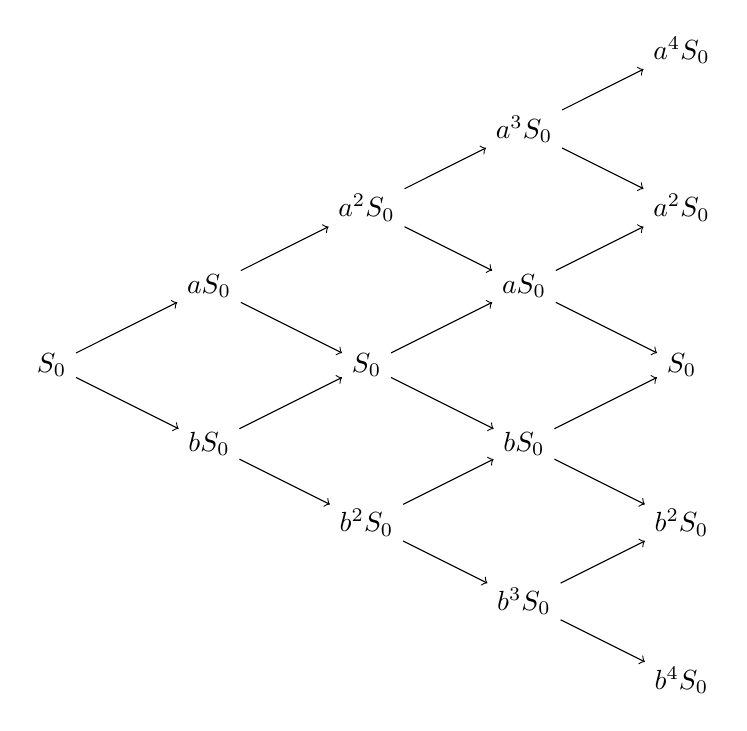
\begin{tikzpicture}
[   cnode/.style={draw=black,fill=#1,minimum width=3mm,circle},
]
\node[] (A) at (0,0) {$S_0$};
\node[] (B) at (2,1) {$aS_0$};
\node[] (C) at (2,-1) {$bS_0$};
\node[] (D) at (4,2) {$a^2S_0$};
\node[] (E) at (4,0) {$S_0$};
\node[] (F) at (4,-2) {$b^2S_0$};
\node[] (G) at (6,3) {$a^3S_0 $};
\node[] (H) at (6,1) {$aS_0 $};
\node[] (I) at (6,-1) {$bS_0 $};
\node[] (J) at (6,-3) {$b^3S_0 $};
\node[] (K) at (8,4) {$a^4S_0$};
\node[] (L) at (8,2) {$a^2S_0$};
\node[] (M) at (8,0) {$S_0$};
\node[] (N) at (8,-2) {$b^2S_0$};
\node[] (O) at (8,-4) {$b^4S_0$};

\draw[->] (A) -- (B);
\draw[->] (A) -- (C);
\draw[->] (B) -- (D);
\draw[->] (B) -- (E);
\draw[->] (C) -- (E);
\draw[->] (C) -- (F);
\draw[->] (D) -- (G);
\draw[->] (D) -- (H);
\draw[->] (E) -- (H);
\draw[->] (E) -- (I);
\draw[->] (F) -- (I);
\draw[->] (F) -- (J);
\draw[->] (G) -- (K);
\draw[->] (G) -- (L);
\draw[->] (H) -- (L);
\draw[->] (H) -- (M);
\draw[->] (I) -- (M);
\draw[->] (I) -- (N);
\draw[->] (J) -- (N);
\draw[->] (J) -- (O);


\end{tikzpicture}
\end{center}

Con los datos del enunciado podemos calcular los valores de $a$ y $b$ mostrados en el esquema, así como la probabilidad de que se de cada suceso. Tomando las fórmulas vistas en los apuntes tenemos:
\[a=e^{σ\sqrt{Δt}} = 1.09, \ b = \frac{1}{a} = 0.92, \ p = \frac{e^{r_cΔt}-b}{a-b}=0.52\]

\spart
Puesto que el valor de la call descrita en el enunciado depende del camino seguido, debemos estudiar los 16 posibles caminos para estudiar, en cada caso, cuál es el valor final del activo. La siguiente tabla recoge los resultados obtenidos:

\begin{center}
\begin{tabular}{|c|c|c|c|}
\hline
\textbf{Trayectoria} & \textbf{Probabilidad} & \textbf{Valor del activo} & \textbf{Valor del derivado}\\
\hline
aaaa & $p^4$        & $a^4S_0$ & $a^4S_0-S_0$ \\
aaab & $p^3(1-p)$   & $a^2S_0$ & $a^2S_0-S_0$ \\
aaba & $p^3(1-p)$   & $a^2S_0$ & $a^2S_0-S_0$ \\
aabb & $p^2(1-p)^2$ & $S_0$ & $0$ \\
abaa & $p^3(1-p)$   & $a^2S_0$ & $a^2S_0-S_0$ \\
abab & $p^2(1-p)^2$ & $S_0$ & $0$ \\
abba & $p^2(1-p)^2$ & $S_0$ & $S_0-bS_0$ \\
abbb & $p(1-p)^3$   & $b^2S_0$ & $0$ \\
baaa & $p^3(1-p)$   & $a^2S_0$ & $a^2S_0-bS_0$ \\
baab & $p^2(1-p)^2$ & $S_0$ & $S_0-bS_0$ \\
baba & $p^2(1-p)^2$ & $S_0$ & $S_0-bS_0$ \\
babb & $p(1-p)^3$   & $b^2S_0$ & $0$ \\
bbaa & $p^2(1-p)^2$ & $S_0$ & $S_0-b^2S_0$ \\
bbab & $p(1-p)^3$   & $b^2S_0$ & $0$ \\
bbba & $p(1-p)^3$   & $b^2S_0$ & $b^2S_0-b^3S_0$ \\
bbbb & $(1-p)^4$    & $b^4S_0$ & $0$ \\
\hline
\end{tabular}
\end{center}

Para calcular el valor futuro de este activo simplemente tenemos que multiplicar el valor del derivado por la probabilidad de alcanzar ese valor y sumar los resultados.

Con un script de python, que puede encontrarse en el apéndice \ref{sec:arbolBin}, calculamos el valor de este activo en el instante final y obtenemos:
\[V_T(X) = 1.18\]

Una vez tenemos este valor, podemos traerlo al presente dividiendo entre $e^{r_cΔt}$, que en este caso sería $e^{0.055\cdot 0.5}$, con lo que obtenemos:
\[V_0(X) = 1.14\]

\spart

Con el mismo razonamiento del apartado anterior tenemos:

\begin{center}
\begin{tabular}{|c|c|c|c|}
\hline
\textbf{Trayectoria} & \textbf{Probabilidad} & \textbf{Valor del activo} & \textbf{Valor del derivado}\\
\hline
aaaa & $p^4$        & $a^4S_0$ & $0$ \\
aaab & $p^3(1-p)$   & $a^2S_0$ & $a^3S_0-a^2S_0$ \\
aaba & $p^3(1-p)$   & $a^2S_0$ & $0$ \\
aabb & $p^2(1-p)^2$ & $S_0$ & $a^2S_0-S_0$ \\
abaa & $p^3(1-p)$   & $a^2S_0$ & $0$ \\
abab & $p^2(1-p)^2$ & $S_0$ & $aS_0-S_0$ \\
abba & $p^2(1-p)^2$ & $S_0$ & $aS_0-S_0$ \\
abbb & $p(1-p)^3$   & $b^2S_0$ & $aS_0-b^2S_0$ \\
baaa & $p^3(1-p)$   & $a^2S_0$ & $0$ \\
baab & $p^2(1-p)^2$ & $S_0$ & $aS_0-S_0$ \\
baba & $p^2(1-p)^2$ & $S_0$ & $0$ \\
babb & $p(1-p)^3$   & $b^2S_0$ & $S_0-b^2S_0$ \\
bbaa & $p^2(1-p)^2$ & $S_0$ & $0$ \\
bbab & $p(1-p)^3$   & $b^2S_0$ & $S_0-b^2S_0$ \\
bbba & $p(1-p)^3$   & $b^2S_0$ & $S_0-b^2S_0$ \\
bbbb & $(1-p)^4$    & $b^4S_0$ & $S_0-b^4S_0$ \\
\hline
\end{tabular}
\end{center}

A partir de esta tabla podemos calcular sin problema el valor futuro del derivado combinando la segunda y la cuarta columna. Una vez tenemos esto, como en el apartado anterior, simplemente lo traemos al presente multiplicando por $e^{-0.055\cdot 0.5}$

Empleando de nuevo el script \ref{sec:arbolBin} tenemos:
\[V_T(X) = 0.90 \implies V_0(X) = 0.88\]
\end{problem}

\begin{problem}[2]
Consideramos un subyacente $S$ que vale hoy 12 y cuya dinámica está descrita por un árbol binomial recombinante de 10 períodos mensuales. La volatilidad del subyacente es del 25\% y el tipo libre de riesgo para el periodo es del 3.5 \% (composición continua). Sea $a$ el coeficiente correspondiente del árbol binomial.

\ppart Calcular el valor de una call europea con una barrrera up-and-out en el nivel $a^8S_0$.
\ppart ¿Qué se puede decir de la opción barrera up-and-in de similares características?
\ppart Calcular el valor de una put europea con una barrera down-and-out en el nivel $a^{-8}S_0$.
\ppart ¿Qué se puede decir de una opción barrera down-and-in de similares características?
\ppart Calcular el precio de una opción barrera digital que paga $1$ a vencimiento si la barrera ha sido alcanzada.

\solution

\doneby{Pedro}

Para poder resolver este ejercicio hay una serie de conceptos que debemos aclarar.

Una opción \concept{up-and-out} es tal que si el activo alcanza un cierto valor conocido como \concept{barrera}, deja de existir.

Este tipo de opciones tiene sentido si estamos construyendo un árbol binomial para estudiar el comportamiento de un activo a un plazo de vencimiento relativamente largo, tal que la parte alta del árbol la consideramos inalcanzable (nuestra intuición nos dice que en el mundo real es imposible que se de esa situación).

Con esta misma idea, existen diferentes opciones con comportamientos equivalentes. Así, tenemos la opción \concept{down-and-out} que deja de existir si el activo toca la barrera, que se encuentra por debajo del valor inicial.

De manera complementaria a estas barreras existes tenemos las opciones \concept{up-and-in} y \concept{down-and-in} que, respectivamente, sólo existen cuando el precio del activo alcanza la barrera.


Los datos que conocemos nada más leer el enunciado son:
\[S_0=12, \ T=0.83, \ Δt = 0.083, \ σ=0.25, \ R_c=0.035\]

con estos datos podemos calcular:
\[a=e^{σ\sqrt{Δt}} = 1.08, \ b = \frac{1}{a} = 0.93, \ p = \frac{e^{r_cΔt}-b}{a-b}=0.5\]

\spart

El caso concreto que concierne a este ejemplo no es más que una call para la que debemos tener en cuenta que si alcanza el precio $a^8S_0$ en algún momento, esta desaparece y el valor final resulta 0.

Puesto que no nos dan un precio de ejercicio $K$ vamos a suponer $K=S_0$\footnote{Esta suposición es correcta y la esperada por el profesor}.

El valor en $t=T$ de la call mencionada sería:
\[V_T(C_K) = \sum_{i=5}^{10}{10 \choose i}a^{i}b^{10-i}p^i(1-p)^{10-i}S_0-S_0\]

Ahora debemos comprobar cuantas de las trayectorias que estamos considerando al calcular $V_T(C_K)$ quedan anuladas por alcanzar el valor $a^8S_0$. Para ello basta con notar que eso ocurre siempre que tengamos 9 o 10 subidas en el proceso de desplazamiento por el árbol o si tenemos 8 subidas consecutivas. En estos casos el valor del activo es 0 en lugar de tener el valor de la Call. Así podemos escribir:
\[V_T(X)=\sum_{i=5}^{8}{10 \choose i}a^{i}b^{10-i}p^i(1-p)^{10-i}S_0-S_0-p^8(1-p)^2(a^6S_0-S_0)\]

Por último, para conocer el valor actual de este activo debemos traerlo al presente mediante un proceso de precios descontados.
\[V_0(X)=V_T(X)e^{-r_cΔt}=V_T(X)e^{-0.035\cdot 0.83}\]

Para realizar esta cuenta utilizamos el script de python \ref{sec:arbolBin} con lo que obtenemos:
\[V_0(X) = 1.449\cdot e^{-0.035\cdot 0.83} = 1.407\]

\spart

En esta ocasión tenemos la misma call del apartado anterior pero la opción de barrera funciona justo al contrario. Necesitamos alcanzar el valor $a^8S_0$ para que el activo esté realmente disponible.

En esta ocasión tendremos:
\[V_T(X)=\sum_{i=9}^{10}{10 \choose i}a^{i}b^{10-i}p^i(1-p)^{10-i}S_0-S_0+p^8(1-p)^2(a^6S_0-S_0)\]
lo que nos lleva a un precio de:
\[V_0(X)=V_T(X)e^{-r_cΔt}=V_T(X)e^{-0.035\cdot 0.83} = 0.1288 \cdot 0.97127 = 0.125\]

donde el resultado numérico se ha calculado con la ayuda del script \ref{sec:arbolBin}
\spart

Este apartado es equivalente al apartado a) pues el árbol que lo representa es el espejo del de este apartado. Por tanto, es sencillo ver que:
\[V_T(P_K) = S_0 -\sum_{i=5}^{10}{10 \choose i}b^{i}a^{10-i}(1-p)^i(p)^{10-i}S_0\]
\[V_T(X) = S_0 -\sum_{i=5}^{8}{10 \choose i}b^{i}a^{10-i}(1-p)^i(p)^{10-i}S_0-(1-p)^8p^2(S_0-b^6S_0)\]
Finalmente
\[V_0(X)=V_T(X)e^{-r_cΔt}=V_T(X)e^{-0.035\cdot 0.83}\]

Para realizar esta cuenta utilizamos el script de python \ref{sec:arbolBin} con lo que obtenemos:
\[V_0(X) = 0.911\cdot e^{-0.035\cdot 0.83} = 0.885\]

\spart

Nuevamente nos encontramos con el caso ``complementario'' del anterior por lo que tendremos:

\[V_T(X) = S_0 -\sum_{i=9}^{10}{10 \choose i}b^{i}a^{10-i}(1-p)^i(p)^{10-i}S_0+(1-p)^8p^2(S_0-b^6S_0)\]

Con el correspondiente
\[V_0(X)=V_T(X)e^{-r_cΔt}=V_T(X)e^{-0.035\cdot 0.83} = 0.0224 \cdot 0.97127 = 0.0218\]
donde el resultado numérico, un vez más, ha sido obtenido mediante el empleo del script \ref{sec:arbolBin}

\spart

No es más que una situación de barrera como las anteriores salvo que en lugar de tener una Call o una Put sobre la que aplicamos la barrera, directamente obtenemos un pago de $1$ si la barrera se ha alcanzado y $0$.

\textcolor{red}{En cuanto pregunte al profesor y me diga que barrera poner podré hacer el ejercicio}

\end{problem}

\begin{problem}[3]
El subyacente $S$ vale hoy 10 y su dinámica está descrita por un árbol binomial recombinante de seis períodos a un horizonte temporal de medio año. La volatilidad del subyacente es del 28\% y el tipo libre de riesgo para el período es del 53\% (composición continua).
\ppart Calcular el precio de una call asiática de media artimética con precio de ejercicio 10
\ppart Misma pregunta para la call de media geométrica
\ppart Qué vale la opción cuyo flujo final viene dado por:
\[(S_0-\frac{1}{6}\sum_{i=1}^6S_i)^+\]
\solution

\doneby{Pedro}


Los datos que conocemos nada más leer el enunciado son:
\[S_0=10, \ T=0.5, \ Δt = 0.083, \ σ=0.28, \ R_c=0.053\]

con estos datos podemos calcular:
\[a=e^{σ\sqrt{Δt}} = 1.08, \ b = \frac{1}{a} = 0.93, \ p = \frac{e^{r_cΔt}-b}{a-b}=0.53\]

\spart

Una \concept{call asiática} de media aritmética es una opción tal que su valor en la fecha de ejercicio es:
\[\max\{0, A(T)-K\}, \text{ donde } A(T) = \frac{1}{n} \sum_{i=1}^nS_{t_i}\]

La forma de hacer este ejercicio consiste en plantear todos los posibles caminos y, para cada camino, calcularemos el precio final de la call y la probabilidad de que se de esa situación. La figura \ref{fig:2_3a} muestra los resultados obtenidos

La tabla ha sido generada por el mismo script, \ref{sec:arbolBin}, que nos permite obtener el siguiente resultado para el valor final de la call:
\[V_1(C) = 2.0161 \implies V_0(C) = 1.9634\]
donde el precio actual de la call se ha calculado mediante un proceso de precios descontados.

\obs Nuevamente, no se especifica el precio de ejercicio de la opción, por lo que asumimos que este es igual al precio actual del activo asociado. Es decir, tomamos por defecto $K=S_0$.

\spart

Cuando tenemos una \concept{call asiática de media geométrica}, la única diferencia respecto a la de media aritmética es la forma en que se calcula la media de los valores que ha tomado el activo para calcular el valor final. Así tenemos que su valor viene dado por la expresión:
\[\max\{0, G(T)-K\}, \text{ donde } G(T) = \sqrt[n]{\prod_{i=1}^nS_{t_i}}\]

De la misma manera que hicimos en el apartado anterior, vamos a estudiar todos los caminos que puede seguir el activo y, para cada uno de ellos calcularemos su valor final y la probabilidad de que se diera esa situación.

La tabla \ref{fig:2_3b} recoje los diferentes caminos explorados y los valores y probabilidades asociados a cada uno.

Con el mismo script de siempre, obtenemos el siguiente resultado:
Ahora sólo tenemos que ponderar los valores calculados con las probabilidades asociadas con lo que obtenemos:
\[V_1(C) = 5.131 \implies V_0(C) = V_1(C)e^{-r_cΔt} = 4.997\]

\spart

Empleando de nuevo nuestro maravilloso script obtenemos los resultados mostrados en la figura \ref{fig:2_3c} que nos lleva a un valor de la opción:
\[V_1(C) = 0.2524 \implies V_0(C) = V_1(C)e^{-r_cΔt} = 0.2458\]
\end{problem}


\begin{problem}[4]
Se considera el subyacente del problema anterior
\ppart Calcular el valor de la opción digital \textbf{cash-or-nothing} que paga $1$ cuando el subyacente esté por encima de $S_0$ a vencimiento.
\ppart Calcular el valor de la opción digital \textbf{asset-or-nothing} que paga una unidad de subyacente a vencimiento cuando este esté por encima de $S_0$.
\solution

\doneby{Pedro}

Los conceptos de opciones \concept{cash-or-nothing} y \concept{asset-or-nothing} quedan definidos claramente en el propio enunciado del ejercicio.

Puesto que estamos utilizando los mismos datos del ejercicio anterior y tenemos:
\[S_0=10, \ T=0.5, \ Δt = 0.083, \ σ=0.28, \ R_c=0.053\]

lo que nos permitía calcular:
\[a=e^{σ\sqrt{Δt}} = 1.08, \ b = \frac{1}{a} = 0.93, \ p = \frac{e^{r_cΔt}-b}{a-b}=0.53\]

Este ejercicio es idéntico al anterior salvo que la forma de calcular el valor final de cada posible ``camino'' es diferente. Aunque este ejercicio podría llevarse a cabo de forma manual puesto que las operaciones son sencillas y es fácil simplificar, empleamos de todas formas el script \ref{sec:arbolBin} para poder generar las tablas correspondientes.

\spart

La figura \ref{fig:2_4a} muestra el estudio de los ``caminos'' asociados a este activo.


Con estas condiciones tenemos
\[V_T(CON) = 0.7106 \implies V_T(CON) = V_1(CON)e^{-r_cΔt} = 0.6983\]

\spart

La figura \ref{fig:2_4b} muestra el estudio de los ``caminos'' asociados a este activo.

Con estas condiciones tenemos
\[V_T(CON) = 8.17204 \implies V_T(CON) = V_1(CON)e^{-r_cΔt} = 8.03027\]

\end{problem}

\begin{problem}[5]
Consideramos un modelo discreto para la dinámica del activo $S$ con $N$ períodos. Sean $C_0$ el valor en 0 de una call de precio de ejercicio $K$, y vencimiento $T$, y $r_c$ el tipo libre de riesgo para composición continua.
\ppart Demostrar que necesariamente $C_0\geq S_0-Ke^{-r_cT}-D$ siendo $D$ el valor actual de los dividendos futuros del subyacente. [sugerencia: suponer que no es así y construir un arbitraje]

\ppart Deducir de ello que, en el árbol binomial, para todo instante $n$, se verifica que $C_n\geq S_n-K(1+r)^{-(N-n)}-D_n$, siendo aquí $D_n$ el valor en $n$ de los dividendos futuros.

\ppart Concluir que, para una call, si el subyacente no paga dividendos, nunca interesa ejercer la opción antes de vencimiento.

\ppart Consideramos ahora el caso de una put de valor $P_n$. Usar la paridad call put para escribir la condición de ejercicio como:
\[K-S_n > C_n-S_n + K(1+r)^{-(N-n)}\]

\ppart Deducir de ello que una CNS de ejercicio es que tengamos:
\[\frac{K\cdot r}{(1+r)^{(N-n)}}> C_n\]
\solution

\end{problem}

\begin{problem}[6]
Usar la fórmula de Cox-Rubinstein y la paridad call-put:
\[C_0=S_0 \phi(n_0,N,q')-\frac{K}{(1+r)^N}\phi(n_0,N,q), \ \ C_0-P_0=S_0-\frac{K}{(1+r)^N}\]
para obtener la fórmula de valoración de la put
\[P_0=\frac{K}{(1+r)^N}\bar{\phi}(n_0,N,q)-S_0\bar{\phi}(n_0,N,q')\]
siendo
\[\bar{\phi}(n_0,N,q)=P(X<n_0) \text{ para } X \approx B(N,q)\]
\solution
\doneby{Pedro}

Despejando $P_0$ de la ecuación de paridad call-put y sustituyendo $C_0$ por su valor en la fórmula de Cox-Rubinstein tenemos

\[P_0 = C_0-S_0+\frac{K}{(1+r)^N} = S_0 \phi(n_0,N,q')-\frac{K}{(1+r)^n}\phi(n_0,N,q)- S_0 + \frac{K}{(1+r)^N} =\]
\[ = \frac{K}{(1+r)^N}\left(1-\phi(n_0,N,q) \right) + S_0\left(\phi(n_0,N,q') -1\right)\]

Una vez llegados a este punto basta con ver que
\[\bar{\phi}(n_0,N,q) = P(X<n_0) = 1- P(x \geq n_0) = 1-\phi(n_0,N,q)\]
con lo que
\[\left(1-\phi(n_0,N,q) \right) = \left(\bar{\phi}(n_0,N,q) \right) \text{ y } \left(\phi(n_0,N,q') -1\right) = \left(-\bar{\phi}(n_0,N,q') \right)\]
con lo que obtenemos exactamente la fórmula de la put.
\end{problem}